\documentclass{article}

\usepackage{../sty/notes}

\usetikzlibrary{decorations.pathmorphing, decorations.markings}
\tikzstyle{mass}=[fill=gray!50, draw, minimum width=2cm, minimum height=1cm]
\tikzstyle{smallmass}=[mass, minimum width=1cm, minimum height=.5cm]
\tikzstyle{wheel}=[circle, fill=gray!25, draw, yshift=-0.25cm, minimum size=0.5cm]
\tikzstyle{spring}=[thick, decorate, decoration={zigzag, pre length=0.3cm, post length=0.3cm, segment length=8}]
\tikzstyle{damper}=[thick, decorate, decoration={markings, mark connection node=dmp, mark=at position 0.5 with
{
    \node (dmp) [thick, inner sep=0pt, transform shape, minimum width=10pt, minimum height=10pt, draw=none, fill=green!20] {};
    \draw [thick] (dmp.south east) -- (dmp.south west) -- (dmp.north west) -- (dmp.north east);
    \draw [thick] (dmp |- dmp.35) -- (dmp |- dmp.-35);
    \draw [thick] (dmp.center) -- (dmp.east);
}
}]


\begin{document}

\section*{Dynamic magnification factor}

The steady state vibration of a \emph{spring}-\emph{mass}-\emph{damper} system depends on the external force applied to it, regadless of the initial conditions. Making use of the steady state solution, the full solution of the vibration can be obtained by adding the transient solution, which satisfies the initial conditions.

\begin{center}
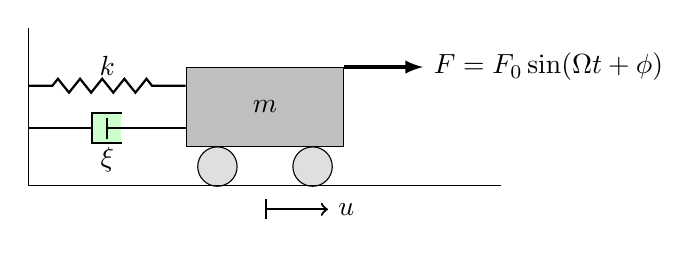
\begin{tikzpicture}
    \coordinate (O);
    \coordinate (U) at (0,-.3);
    \node [mass] (m) at (3,1) {$m$};
    \node [wheel] at (m.220) {};
    \node [wheel] at (m.320) {};
    \draw [spring] (m.165 -| O) -- (m.165) node [midway,above] {$k$};
    \draw [damper] (m.195 -| O) -- (m.195) node [midway,below=3pt] {$\xi$};
    \draw [very thick,-latex] (m.north east) -- ++(1,0) node [right] {$F=F_0\sin(\Omega t + \phi)$};
    \draw (O) -- (0,2);
    \draw (O) -- (6,0);
    \draw [|->,thick] (m |- U) -- ++(.8,0) node [right] {$u$};
\end{tikzpicture}
\end{center}

The governing equation of motion for the steady state solution is given by
$$
\ddot{u} + 2\xi\omega\dot{u} + \omega^2u = \frac{F}{m}
$$

Taking a trial function $u=\frac{F_0}{k}H\sin(\Omega t + \phi - \Delta\phi)$, the response is given by
$$
\frac{F_0}{k}H\left(
    (\omega^2-\Omega^2)\sin(\Omega t + \phi - \Delta\phi) + 2\xi\omega\Omega\cos(\Omega t + \phi - \Delta\phi)
\right) = \frac{F_0}{m} \sin(\Omega t + \phi).
$$
Using the notation $\gamma=\Omega/\omega$ and making use of the composition rule for sine and cosine functions, the previous expression leads to
$$
H\sqrt{(1-\gamma^2)^2 + 4\xi^2\gamma^2} \sin\left(\Omega t + \phi -\Delta\phi + \tan^{-1}\frac{2\xi\gamma}{1-\gamma^2}\right) =
    \sin(\Omega t + \phi)
$$

Finally, the dynamic magnification factor and phase lag are
\begin{align*}
    &H = \frac{1}{\sqrt{(1-\gamma^2)^2 + 4\xi^2\gamma^2}} \\
    &\tan\Delta\phi = \frac{2\xi\gamma}{1-\gamma^2}
\end{align*}


\section*{Tuned mass damper}

A tuned mass damper (TMD) consist on a small \emph{spring}-\emph{mass}-\emph{damper} system attached to the main system.

\begin{center}
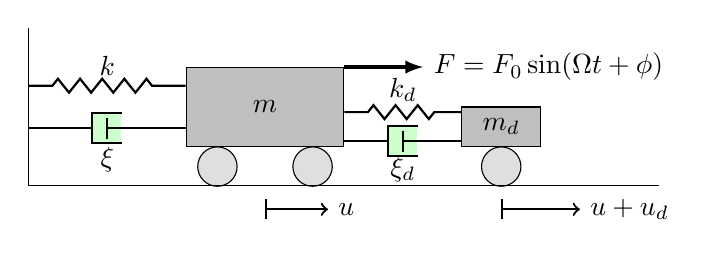
\begin{tikzpicture}
    \coordinate (O);
    \coordinate (U) at (0,-.3);
    \node [mass] (m) at (3,1) {$m$};
    \node [wheel] at (m.220) {};
    \node [wheel] at (m.320) {};
    \draw [spring] (m.165 -| O) -- (m.165) node [midway,above] {$k$};
    \draw [damper] (m.195 -| O) -- (m.195) node [midway,below=3pt] {$\xi$};
    \draw [very thick,-latex] (m.north east) -- ++(1,0) node [right] {$F=F_0\sin(\Omega t + \phi)$};
    \node [smallmass] (md) at (6,.75) {$m_d$};
    \node [wheel] at (md.south) {};
    \draw [spring] (md.160 -| m.east) -- (md.160) node [midway,above] {$k_d$};
    \draw [damper] (md.200 -| m.east) -- (md.200) node [midway,below=2pt] {$\xi_d$};
    \draw (O) -- (0,2);
    \draw (O) -- (8,0);
    \draw [|->,thick] (m |- U) -- ++(.8,0) node [right] {$u$};
    \draw [|->,thick] (md |- U) -- ++(1,0) node [right] {$u+u_d$};
\end{tikzpicture}
\end{center}

Here, the subscript $d$ refers to the tuned mass damper and the following notation is introduced,
\begin{align*}
    \omega^2 &= \frac{k}{m} \\[2pt]
    \omega^2_d &= \frac{k_d}{m_d} \\[2pt]
    \gamma &= \frac{\Omega}{\omega} \\[2pt]
    \rho &= \frac{m_d}{m} \ll 1 \\[2pt]
    \eta &= \frac{\omega_d}{\omega} \approx 1
\end{align*}

The governing equations of motion for the steady state solution are given by
\begin{align*}
(1+\rho)\ddot{u} + 2\xi\omega\dot{u} + \omega^2 u = \frac{F}{m} - \rho\ddot{u}_d & \qquad \text{(primary mass)} \\
\ddot{u}_d + 2\xi_d\omega_d\dot{u} + \omega^2u_d = -\ddot{u} & \qquad \text{(tuned mass)}
\end{align*}

\subsection*{\colorbox{lightgray}{$\xi=0$} Undamped structure, damped TMD}

Using the trial functions
\begin{align*}
    u &= \frac{F_0}{k}\bar{H}e^{i\Omega t} \\[2pt]
    u_d &= \frac{F_0}{k}\bar{H}_de^{i\Omega t}
\end{align*}
the response is given by
\begin{gather*}
    -(1+\rho)\Omega^2\frac{F_0}{k}\bar{H}e^{i\Omega t} + \omega^2\frac{F_0}{k}\bar{H}e^{i\Omega t} =
        \frac{F_0}{m}e^{i\Omega t} + \rho\Omega^2\frac{F_0}{k}\bar{H}_de^{i\Omega t} \\
    -\Omega^2\frac{F_0}{k}\bar{H}_de^{i\Omega t} + i2\xi_d\omega_d\Omega\frac{F_0}{k}\bar{H}_d e^{i\Omega t} +
        \omega_d^2\frac{F_0}{k}\bar{H}_de^{i\Omega t} = \Omega^2\frac{F_0}{k}\bar{H}e^{i\Omega t}
\end{gather*}
which yields the following expression, after simplification and cancelling the $e^{i\Omega t}$ terms
\begin{gather*}
    \bar{H} - (1+\rho)\gamma^2\bar{H} = 1 + \rho\gamma^2\bar{H}_d \\
    \eta^2\bar{H}_d - \gamma^2\bar{H}_d + i2\xi_d\gamma\eta\bar{H}_d = \gamma\bar{H}
\end{gather*}

The solution is
\begin{gather*}
    \bar{H} = \frac{\eta^2 - \gamma^2 + i2\xi_d\gamma\eta}{\bar{H}^*} \\
    \bar{H}_d = \frac{\gamma^2}{\bar{H}^*} \\
\end{gather*}
with
$$
\bar{H}^* = (\eta^2-\gamma^2)(1-\gamma^2) - \rho\gamma^2\eta^2 + i2\xi_d\gamma\eta(1-\gamma^2(1+\rho))
$$

The complex numbers $\bar{H}$ and $\bar{H}_d$ are definig a modulus $H$ and a phase angle $\Delta\phi$, both for the primary and the tuned mass. The real and imaginary parts correspond to a cosine and sinusoidal functions, so the polar form can be converted into a trigonometric function,
\begin{gather*}
    u = \frac{F_0}{k}H\sin(\Omega t + \Delta\phi - \Delta\phi_d) \\
    u_d = \frac{F_0}{k}H_d\sin(\Omega t - \Delta\phi_d) \\
\end{gather*}

For the primary mass we have
$$
H = \sqrt{\frac{(\eta^2-\gamma^2)^2 + 4\xi_d^2\gamma^2\eta^2}
    {((\eta^2-\gamma^2)(1-\gamma^2)-\rho\gamma^2\eta^2)^2 + (2\xi_d\gamma\eta(1-\gamma^2(1+\rho)))^2}}
$$
\begin{align*}
    \tan\Delta\phi &= \frac{2\xi_d\gamma\eta}{\eta^2-\gamma^2} \\
    \tan\Delta\phi_d &= \frac{2\xi_d\gamma\eta(1-\gamma^2(1+\rho))}{(\eta^2-\gamma^2)(1-\gamma^2) - \rho\gamma^2\eta^2}
\end{align*}

Figure \ref{H-gamma_eta} shows several response function at different tuned frequencies. It can be seen that the optimal TMD is achieved when the two maximums of $H$ are symmetrics. It happens at
$$
\eta_\text{opt} = \frac{1}{1+\rho}
$$

Once the optimal tuned frequency is set, the tuned damping can modify the response. An excessive damping ratio may generate a monolitic response while a low damping ratio exibits two peaks of ressonance. Figure \ref{H-gamma_xi} shows the response, the optimal damping ratio is
$$
\xi_\text{opt}^2 = \frac{\rho(3-\sqrt{0.5\rho})}{8(1+\rho)(1-0.5\rho)}
$$

\begin{figure}
    \centering
    \includegraphics[width=.8\textwidth]{tmd-frequencies.pdf}
    \caption{Plot of dynamic magnification factor $H$ versus forcing frquency $\gamma$ at different tuning frequencies $\eta$. The shadowed region shows dynamic magnification without TMD.}
    \label{H-gamma_eta}
\end{figure}


\begin{figure}
    \centering
    \includegraphics[width=.8\textwidth]{tmd-dampings.pdf}
    \caption{Plot of dynamic magnification factor $H$ versus forcing frquency $\gamma$ with different tuned dampings $\xi_d$. The shadowed region shows dynamic magnification without TMD.}
    \label{H-gamma_xi}
\end{figure}

\end{document}
